\section{Introduction}
% abstract + intro fill first page

% information society, modern, communication, integral part of daily life, substantial amounts of data, prior research either topics or networks (not both)

In our modern information society, we produce substantial amounts of data each day, where a large portion of it comes from the communication through social media platforms or email.
Given a dataset of the exchanged information over a year, it is practically impossible to gain an overview or quick insights into the data.
Journalists for example find themselves in this position whenever they receive huge collections of leaked data.
A system that automatically generates an interactive overview of latent structures and topics may support the search for potential stories and identify relevant documents.

In this paper, we propose an interactive visualisation that positions individuals on a two-dimensional canvas such that it reflects their community in which they communicate as well as the topical relatedness.
To do so, we utilise document embeddings which project the content of a message into a high dimensional semantic space as well as node2vec, which projects nodes in a network graph into a latent space reflecting similar connectivity.

%In recent years, research has enabled us to position words or even entire documents in a high dimensional semantic space and visualise it on a two-dimensional plane.
%Similarly, there is a multitude of approaches to layout a network graph to convey coherent structures.

% related work
% - topic maps/topic vis/textvis
% - network vis
% TODO: cite simething from nikos bikakis (http://www.dblab.ntua.gr/~bikakis/)
% ( organises the workshop )
\cite{chen2009exemplar}
\cite{dang2017cactustree}
\cite{efrat2015mapsets}
\cite{fortuna2005visualization}
\cite{fried2014maps}
\cite{gronemann2012drawing}
\cite{hildenbrand2016flexible}
\cite{pang2017creating}
\cite{sallaberry2016contact}
\cite{sen2017cartograph}
\cite{tao2017honvis}
\cite{wei2010tiara}
\cite{white2009exploratory}
\cite{yang2014overlapping}

related work
\begin{itemize}
	\item two parts: network vis, textvis
	\item embeddings: doc2vec, node2vec
	\item hierarchical/level of detail
	\item map semantic
	\item cartograph close to us, but no network
	\item highlight missing link between text and network in all research
\end{itemize}

Lorem ipsum dolor sit amet, consectetur adipiscing elit. Quisque sed massa enim. Nullam efficitur urna vel aliquam suscipit. Mauris feugiat ut mauris vitae ultrices. Nam varius velit eu fringilla tempus. Quisque non nunc sem. Donec porta odio sit amet ante rutrum ullamcorper. Vivamus ac mauris blandit, rutrum neque et, suscipit urna. Sed commodo scelerisque sapien. Quisque ullamcorper velit sit amet molestie iaculis. Nullam at erat justo. Nulla in erat luctus, condimentum elit et, posuere enim. Nullam ut ex in massa dignissim vulputate at nec mauris. Donec cursus nibh sed libero posuere, a molestie risus pulvinar. Sed iaculis ante lacinia varius pretium. Suspendisse euismod arcu vel ex dignissim tristique. Mauris sed ex eu nisi efficitur faucibus at in libero.

Praesent purus mauris, auctor eget viverra et, rhoncus in nisi. In ut sagittis nulla. Pellentesque fringilla enim leo, nec tempor dolor mollis et. Proin sed rutrum orci. Nulla imperdiet et purus at ornare. Etiam quis dictum erat. Maecenas aliquet vel erat in hendrerit. Aenean a purus sit amet odio placerat tempus. Quisque quis eros odio. Nulla eu accumsan nulla.

Praesent porttitor nulla sit amet neque aliquet vestibulum. Cras nec tellus augue. Suspendisse tincidunt sapien luctus, feugiat nisi nec, venenatis lorem. In aliquet id velit ut vulputate. Vestibulum aliquet interdum dui molestie interdum. Cras pretium bibendum justo. Phasellus congue laoreet turpis, at tincidunt ante fermentum vitae. Cras id nisi at lorem hendrerit dictum eget ullamcorper ipsum. Donec vulputate id urna quis interdum.

Class aptent taciti sociosqu ad litora torquent per conubia nostra, per inceptos himenaeos. Ut sit amet cursus neque, volutpat tempus lacus. Cras ultricies enim eu ipsum bibendum eleifend. Donec gravida, sapien id pellentesque faucibus, mi diam pharetra ipsum, non pretium justo ante a ante. In ut accumsan ante. Aenean tempus egestas metus, quis laoreet nisl porta in. Phasellus sed sem vitae nisi egestas ullamcorper. Integer pellentesque nisl erat, quis imperdiet neque aliquet vel. Cras sollicitudin, orci quis interdum ullamcorper, nunc sapien dapibus dui, ut lobortis tellus lorem ac mi. Aenean risus orci, iaculis sed mattis sed, fringilla vitae lectus. Phasellus ac metus mollis, maximus magna sed, porta ligula.

Pellentesque ac lorem lorem. Nulla suscipit nulla id eros blandit, eget eleifend ipsum euismod. Duis nulla turpis, egestas ut lacus non, ultrices iaculis velit. Duis tincidunt volutpat dolor, vel tempor ante laoreet at. Sed ultricies magna nec enim feugiat ullamcorper. Maecenas iaculis laoreet lorem eget vehicula. Quisque dignissim nisi urna, egestas venenatis erat malesuada non. Nullam vel metus in arcu dictum egestas a nec velit. Morbi lorem ex, luctus a maximus id, blandit id ex. Duis libero orci, consectetur ut erat sed, finibus convallis elit. Curabitur vitae orci eu sapien sodales tempor.

Pellentesque ac lorem lorem. Nulla suscipit nulla id eros blandit, eget eleifend ipsum euismod. Duis nulla turpis, egestas ut lacus non, ultrices iaculis velit. Duis tincidunt volutpat dolor, vel tempor ante laoreet at. Sed ultricies magna nec enim feugiat ullamcorper. Maecenas iaculis laoreet lorem eget vehicula. Quisque dignissim nisi urna, egestas venenatis erat malesuada non. 

%introduce topic, challenges, rough goal, related work

\begin{figure*}
	% alternatively use teaserfigure (manual page 18)
	% A special kind of figure is used for many two-column conference proceedings. This figure is placed just after the authors, but before the main text. The environment teaserfigure is used for these figures. This environment must be used before \maketitle
	%\dummyfig{0.3}{0.8}{mockup}
	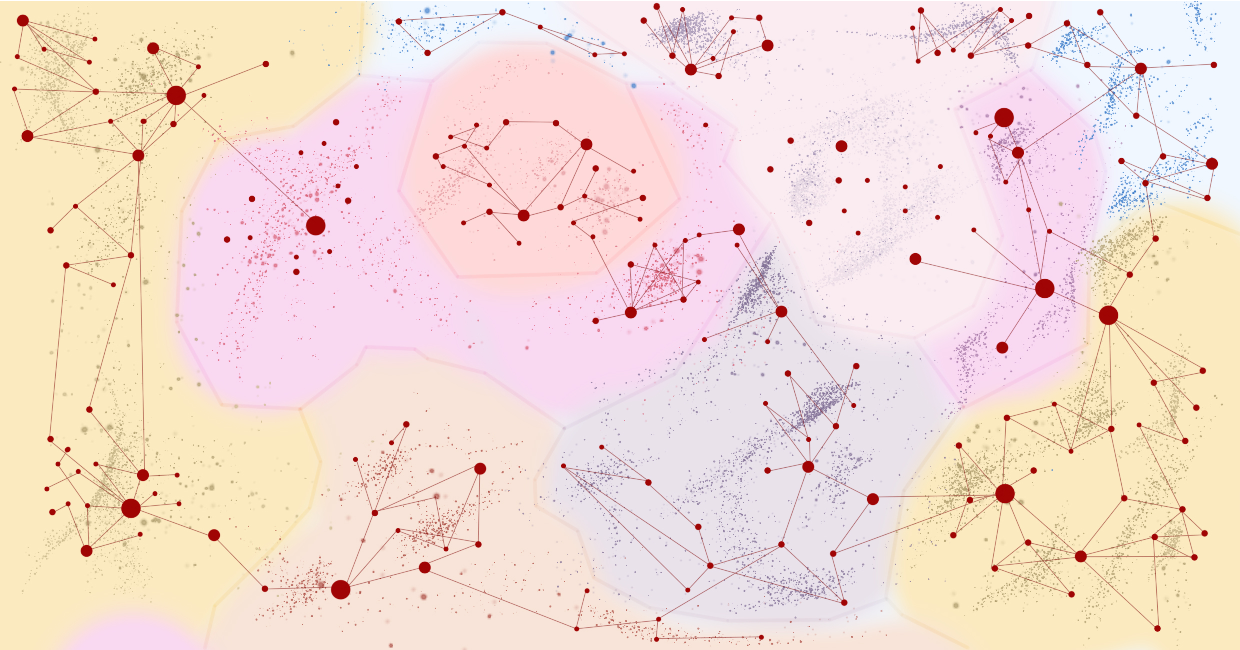
\includegraphics[width=0.9\textwidth]{mockup2}
	\caption{Semantic landscape of email contents and dominant communication patterns (drawn mockup)}
	\label{fig:mockup}
\end{figure*}



\section{Interactive Visualisation}
% this section fills second page (inkl mockup)
% describe objectives and what data is available and how that can be used
Systems for document exploration largely vary in what they display and how the user interacts with them, which is already reflected in the way the data is preprocessed or enriched with external sources. 
The design is primarily dictated by the objectives users have.

We distinguish between a bottom-up approach, in which a user initiates an exploration from a specific document or entity, and a top-down approach, in which the system provides an abstract overview of the entire document collection and the user incrementally refines the search narrowing in to just a few documents.
While a bottom-up approach can provide detailed information from the start, it requires a-priori knowledge by the user.
In contrast, the top-down approach can help a user without prior knowledge to get a sense for the data by visualising high level latent structures of the communication network or the topical distribution.

In the scope of this work we primarily consider documents to be emails or data attached to them.
The sender, recipients, time, and content can directly be extracted from the raw data.
We call these -- and results from further processing -- \textit{dimensions} that can be visualised.
From the contents one may infer named entities, topics, embeddings, or salient phases from the content, while the communication network spanned by sender-recipient pairs can be used to detect salient structures and hierarchies.
The temporal information enables the previously mentioned data to be analysed over time to detect evolving or changing patterns.

There are numerous ways to visualise each dimension on its own or as a combination of many.
The user's objective implies which dimension is needed, optional, or irrelevant and also which priority each dimension gets in the visualisation.
From the wide range of possibilities, we strive for a system which helps journalists or investigators to explore a large collection of documents without any prior knowledge about the content and individuals involved.

Thus, we consider the names or email addresses of senders and recipients (from now on \textit{individuals}), the communication network, semantic vector representations of email contents, and as part of an overlay the timestamps of emails.
\Fref{fig:mockup} shows a manually drawn mockup of the system we are working on.

The individuals are represented as nodes positioned such that densely connected communities are visually clustered.
Edges describe the email traffic, where the opacity and thickness is used to indicate the frequency of messages between the nodes they connect.
The semantic representations of emails are used to place dots on a background layer which we call the \textit{document landscape}.
This landscape is used as additional input to the graph layout algorithm, aiming to place a node within corresponding semantic regions.
The colouring of regions in the landscape is derived from densely connected communities in the communication graph.
We select representative words for densely populated areas in the landscape, so that users get a rough idea about subjects in that area.
The aforementioned timestamps of emails can be used to generate a heatmap overlay to show the activity in a certain time interval which is controlled by a slider.

Similar to modern geographical maps, zooming into a region reveals more details.
In our case, less prominent individuals and their connections are shown along with additional salient phrases from the document landscape.
Selecting a node will not only highlight connected edges but may also temporarily show more edges which were previously hidden at that zoom level.
The user will also be able to retrieve documents with the help of a selection rectangle or clicking dots in the document landscape.

%We further distinguish between domain oriented and open systems. 
%A domain oriented system may have specific vis, extract, ext data,...


\section{System Architecture}
% fills full page 3 and max the first half of left column page 4
%describe concrete system and outline algorithmic approach
Visualising communication networks in a topic-aware fashion to explore documents and salient structures is not straight forward, as different layout objectives may produce contradicting results.
In this section, we describe algorithmic approaches behind the system we are working on.
For a discussion of engineering aspects on how to store, serve, and render the map-like data, we refer to the Cartograph~stack~\cite{sen2017cartograph}, as we will focus on the process how to extract the information that the map is generated from.
% self citation -> quagga for preprocessing?

As described in the previous section, we visualise the embedded emails as dots in a two-dimensional landscape in which individuals are placed as nodes connected by edges.
By reducing all emails between two individuals into one edge, we reduce the visual complexity of the network, which makes it easier to detect salient structures.
However, that comes with the trade-off, that nodes and edges cannot be perfectly placed in the landscape to cover all semantic aspects of the communication between them, but rather an estimate.

Our proposed algorithm to find a stable network layout has three stages, namely an \textit{(i) initialisation phase} which creates the landscape and roughly places nodes and connections, an \textit{(ii) update phase} which iteratively updates the node placement towards a better fit, and finally a \textit{(iii) post processing phase} where edges become splines to better match the landscape.

%One na\"ive approach to combine a flat visualisation of the document embedding space and communication graph is to assume the embedded emails to be fixed and place the nodes of the graph close to where most emails are projected to.
%This way, many edges may cross each other and communities can't be visually distinguished.
%Furthermore, in case emails of an individual contain two dominant subjects which are far apart in the semantic space, ideal placement of the node becomes ambiguous.

%We assume, that the communication between two individuals 

%optimise towards
%stable balance

\paragraph{Initialising the Landscape.}
First, we need to generate the document landscape.
Therefore, we train document embeddings~\cite{le2014distributed,hu2017} over all emails and use these embeddings to infer high dimensional semantic vector representations for each email.
These vectors are then reduced in dimensionality using t-SNE~\cite{maaten2008visualizing}, which retains possible clustering of emails in the higher dimensional space and can be used to place them onto a two-dimensional map.
The size of a dot printed on the map is determined by the number of recipients of that email.

We also need to initialise the layout of the communication network.
The staring position of a node representing an individual is determined by summing up the two-dimensional vectors of all emails he or she sent or received normalised by the absolute number.
This way, we not only place a node in the semantically relevant region but also implicitly group related individuals into communities as frequent communication biases this normalised sum.
Straight edges are added between the nodes if the respective individuals exchanged emails.
Note, that in the Enron corpus, many edges only represent a small number of emails.
Applying a variable threshold can reduce the computational load in later stages, as these edges will not impact the overall layout very much.
They can be added again as the user requests a detailed visualisation by zooming in or other interactions.

%filter low freq, no influence on layout

Lastly, we apply node2vec~\cite{grover2016node2vec} to the communication graph, as it will be used to measure the neighbourhood similarity between two nodes in later stages of the algorithm.

\paragraph{Adjusting the Network Layout.}
The first stage of our proposed algorithm produces a fixed document landscape and roughly fits the communication network on top. 
We now aim to incrementally adapt the layout of the graph to better reflect salient structures in the network and aligning the edges to the contained emails in the landscape.
Therefore we define a score quantifying how well the current layout fits these objectives:
\begin{equation}
\sum_{n}^{nodes}\left[\sum_{m}^{\substack{emails\\from~n}}\frac{len(E(n, R(m)))}{sim(n, R(m))}\theta+dist(m, E(n,R(m)))\eta\right]
\label{eq:score}
\end{equation}

where $R(m)$ is the recipient of email $m$, $len$ the length of an edge $E$, $sim$ the node2vec based similarity reflecting the neighbourhood affiliation, and $dist$ the shortest distance from the email $m$ to an edge. The parameters $\theta$ and $\eta$ are used to adjust the layout towards a better semantic or structural fit respectively.

\begin{figure}
	% alternatively use teaserfigure (manual page 18)
	% A special kind of figure is used for many two-column conference proceedings. This figure is placed just after the authors, but before the main text. The environment teaserfigure is used for these figures. This environment must be used before \maketitle
	\dummyfig{0.15}{0.2}{post init example}
	\dummyfig{0.15}{0.2}{post layout example}
	%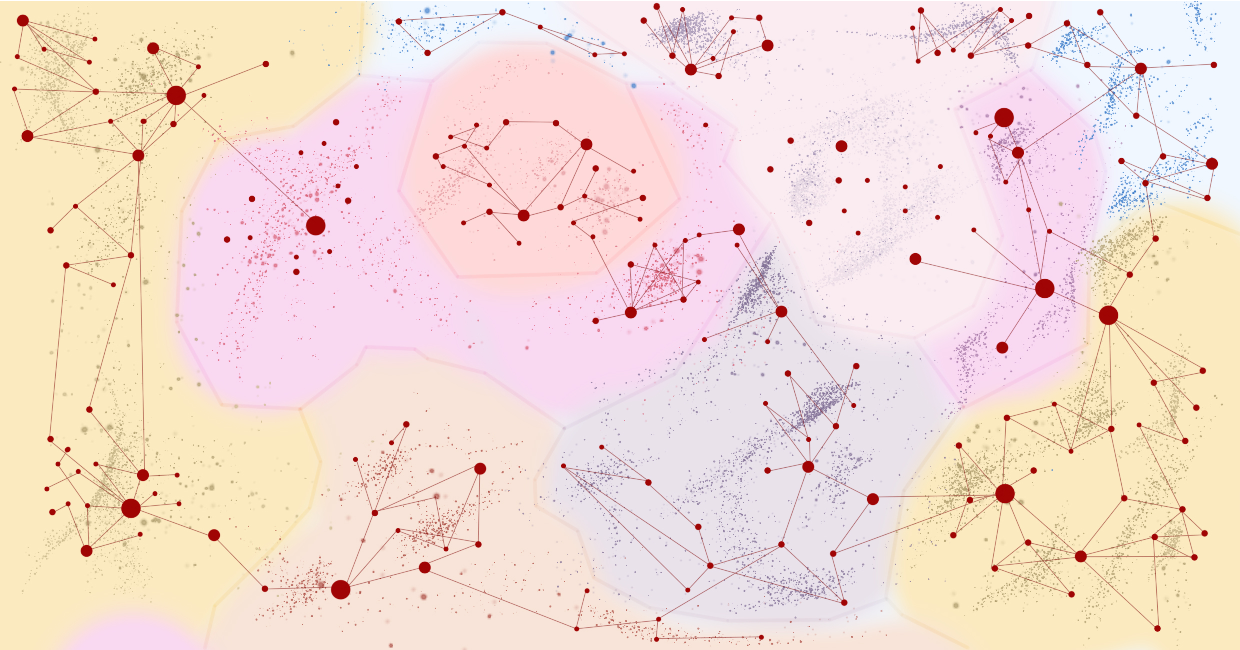
\includegraphics[width=0.9\textwidth]{mockup2}
	\caption{Schematic example after initialisation (left) and after layout optimisation (right). Nodes and edges of the graph are blue, green dots are embedded emails, dotted lines are email--edge relationships, arrows are update vectors}
	\label{fig:minisample}
\end{figure}

\Fref{fig:minisample} schematically shows a small possible scenario after initialisation.
There, the network layout does not yet reflect our objectives very well as communities are spread apart and mixed.
We incrementally move the nodes towards a stable minimum of \Fref{eq:score}.
The direction 

\paragraph{Post Processing.}
bend and bundle edges, calculate network "topology" (community density as heatmap or topological lines), colour the graph (using topic clustering in case layout isn't close to landscape or community colouring if communities aren't visually close enough -> future research)

%parts of the system: prep, server, frontend
%\begin{itemize}
%\item node2vec
%\item node clustering/communities
%\item doc2vec
%\item tsne for docs in cluster
%\item find stable layout
%\item calculate metric for node importance
%\item calculate metric for salient phrases
%\item use last three for map generation with zoom levels
%\item mapserver, database, leaflet (see cartograph)
%\end{itemize}
%
%describe idea of fully neural approach: feed doc2vec and node2vec to second stage network, use that representation only; discuss outcome (nice because fully semantic and no intervention, bad because outcome unpredictable and potentially visually not practical)

\section{Conclusion and Future Work}
% fills left column on page 4, right column mostly references
\begin{itemize}
	\item nice app of big data to find salient communication structures in semantic space
	\item highlight contribution (combine network vis and text vis)
	\item future: implement it, refine algorithm, evaluate usefulness
\end{itemize}